\chapter{Architettura di sistema}

Affinché l'utente sia agevolato nello sviluppo di un firmware esso deve sfruttare al meglio l'interoperabilità dei componenti e le potenzialità dell'intero sistema di sviluppo.

Risulta quindi necessaria una visione di insieme dell'intero sistema invece che una valutazione locale dei singoli componenti. Risulta inoltre necessaria una valutazione della compatibilità intercomponente affinché la loro interazione permetta allo sviluppatore di operare con facilità.

\begin{figure}[t]
    \centering
    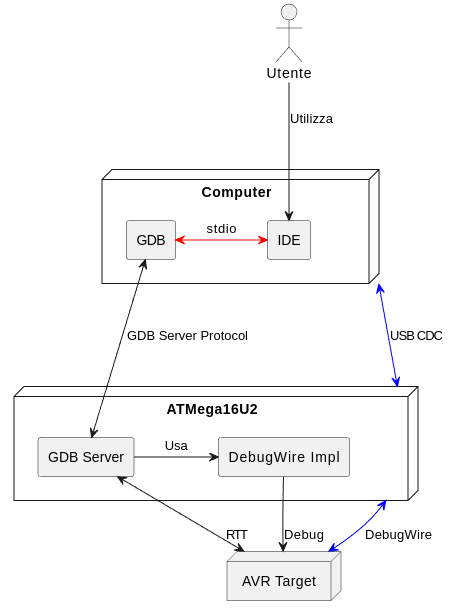
\includegraphics[width=.7\textwidth]{sys-arch.png}
    \caption[]{Diagramma dei componenti del sistema di assistenza alla programmazione e debugging}\label{fig:sys-arch}
\end{figure}

Come osservabile dalla figura~\ref{fig:sys-arch}, il sistema sviluppato si basa su tre livelli fisici collegati a cascata, in modo tale da adattare le azioni ad alto livello scelte dall'utente ai comandi di debug a basso livello che permettono di interagire con il controllore \textit{target}. 

Il primo livello, ovvero il livello di interfaccia con lo sviluppatore, consiste nel software utilizzato per lo sviluppo del firmware contenente tutti gli strumenti di supporto alla programmazione C. Questi software, anche noti IDE\footnote{Integrated Development Environment}, hanno il compito di accorpare svariate funzionalità mediante integrazione di software esterni allo scopo di favorire lo sviluppo fornendo un ambiente unico e integrato allo sviluppatore, dal quale effettuare tutte le operazioni quali sviluppo, compilazione, debugging e upload.

Enfasi particolare viene posta sull'integrazione da parte dell'IDE del software GDB.\@

Il \textit{debugging} è una delle pratiche ormai fondamentali della programmazione la quale permette una comprensione agevolata del flusso di esecuzione del codice e permette di ispezionarne i vari stati.

In particolare esso permette di analizzare uno stato intermedio tramite l'esecuzione in modo interattivo, consentendo allo sviluppatore di condurre ``un'indagine'' relativa a un funzionamento inatteso del firmware. Per citare un detto diffuso sulle piattaforme social in ambito di programmazione possiamo affermare che la procedura di \textit{debugging} sia paragonabile ad un'indagine condotta dallo sviluppatore dove egli stesso è il colpevole.

È necessario porre un'ulteriore enfasi sull'aggettivo ``interattivo'': la differenza tra \textit{debugging} e \textit{logging} sta proprio nel fatto che il secondo consiste solamente nella stampa, su un terminale o file, di una serie di messaggi statici e predefiniti al fine di tracciare gli eventi per un'analisi futura e inaspettata. Ciò non permette quindi di effettuare decisioni in funzione dei risultati parziali ottenuti nella procedura di \textit{debugging} a meno di riprogrammare il dispositivo --- inficiando così sulla longevità delle memorie --- e ricapitolare l'esecuzione del codice.

Risulta quindi di grande importanza poter accedere a uno (o più) software per il debugging in modo che esso possa essere efficiente.
Uno dei software più utilizzati per il debugging del software compilato, qualunque sia il linguaggio scelto, è Gnu GDB\cite{site:gdb}.

\section{Gnu Debugger}\label{sec:gdb}

Il software GDB è un debugger multiarchitettura\cite{site:gdb} utilizzato per l'ispezione degli stati di esecuzione dei software compilati.
In particolare esso presenta un'architettura multipla di funzionamento in funzione della localizzazione del processo da ispezionare.

Generalmente il processo da analizzare è direttamente localizzato sulla stessa macchina nella qualle il processo GDB viene istanziato. In questo caso è sufficiente utilizare delle chiamate di sistema (\textit{syscall}) in grado di accedere e bloccare l'esecuzione del processo da parte del sistema operativo.
Sarà dunque possibile modificare il contenuto della porzione di memoria in cui è caricato l'eseguibile in modo da sostituire l'istruzione incriminata con un'istruzione di ``\textit{break}''. Questa istruzione causerà, al momento della sua esecuzione, un'eccezione a livello hardware la quale verrà gestita dal kernel e notificherà il processo \textit{debugger} che il processo \textit{debuggee} ha raggiunto un \textit{breakpoint}.

Purtroppo non sempre il processo \textit{debuggee} è in esecuzione sullo stesso processore. Questo comporta la necessità di scindere in due componenti il programma utilizzato per effettuare il \textit{debug} adottando un'architettura client-server per consentire la dislocazione del processo \textit{debuggee}.

\subsection{Debugging di dispositivi embedded}

Quanto enunciato precedentemente si avvera nel debugging di dispositivi embedded. 

Possiamo vedere il firmware in esecuzione sul microcontrollore come un processo dislocato su un processore remoto con una diversa architettura.

La problematica relativa la diversa architettura dei processori non costituisce motivo di preoccupazione in quanto ormai la maggior parte degli instruction set è stata inclusa nella distribuzione di GDB multi-architettura[todo cite].
La vera problematica si ha con il la scarsa connettività dell'integrato, la quale richiede un protocollo e un componente di adattamento \textit{ad-hoc}.
L'architettura client-server permette quindi di implementare tale adattatore su un dispositivo esterno connesso con il \textit{target} con possibilità di implementare il protocollo di debug permettendo così di adattare l'interfaccia a tutti i dispositivi in grado di eseguire GDB.

Possiamo vedere come la concezione di separazione tra applicativo di controllo ed interazione e esecutore dei comandi di debug può essere implementata dalla figura~\ref{fig:gdb-server-tunnels}.

\begin{figure}
    \centering
    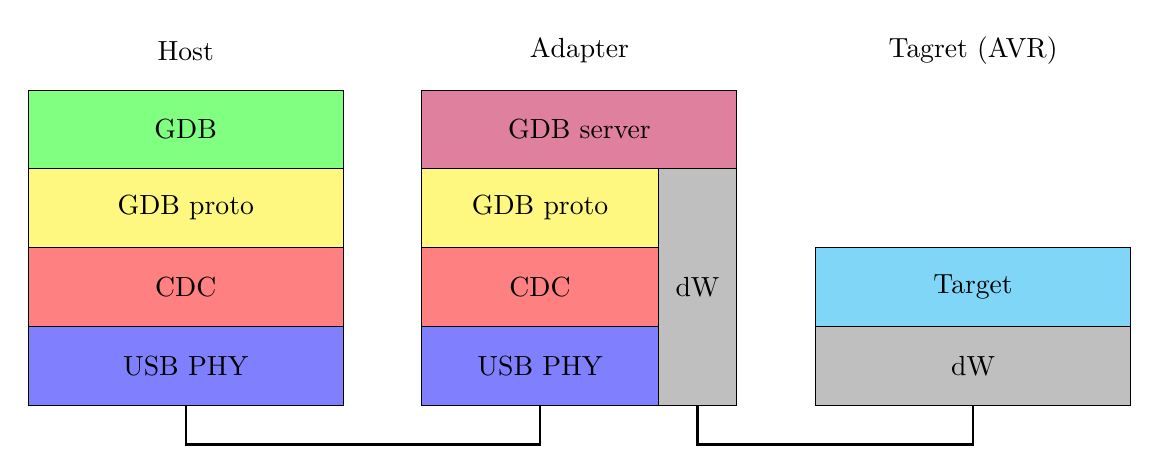
\begin{tikzpicture}
        \draw[fill=green!50] (0,3) rectangle (4,4) node[pos=.5] {GDB}; %GDB
        \draw[fill=yellow!50] (0,2) rectangle (4,3) node[pos=.5] {GDB proto}; %gdb_proto
        \draw[fill=red!50] (0,1) rectangle (4,2) node[pos=.5] {CDC}; %cdc
        \draw[fill=blue!50] (0,0) rectangle (4,1) node[pos=.5] {USB PHY}; %usb_phy
        
        \draw[fill=purple!50] (5,3) rectangle (9,4) node[pos=.5] {GDB server}; %GDB_SERVER
        \draw[fill=yellow!50] (5,2) rectangle (8,3) node[pos=.5] {GDB proto}; %gdb_proto
        \draw[fill=red!50] (5,1) rectangle (8,2) node[pos=.5] {CDC}; %cdc
        \draw[fill=blue!50] (5,0) rectangle (8,1) node[pos=.5] {USB PHY}; %usb_phy
        \draw[fill=gray!50] (8,0) rectangle (9,3) node[pos=.5] {dW}; %dw

        \draw[fill=cyan!50] (10,1) rectangle (14,2) node[pos=.5] {Target}; %AVR
        \draw[fill=gray!50] (10,0) rectangle (14,1) node[pos=.5] {dW}; %dw

        \draw[black, thick] (2, 0) -- (2, -0.5) -- (6.5, -0.5) -- (6.5, 0);
        \draw[black, thick] (8.5,0) -- (8.5, -0.5) -- (12, -0.5) -- (12, 0);

        \node (5) at (2, 4.5) {Host};
        \node (5) at (7, 4.5) {Adapter};
        \node (5) at (12, 4.5) {Tagret (AVR)};
    \end{tikzpicture}
    \caption[]{Diagramma di incapsulamento e protocolli di comunicazione tra debugger e target}\label{fig:gdb-server-tunnels}
\end{figure}

In particolare, la figura rappresenta la scelta intrapresa per lo sviluppo del sistema in esame. È possibile notare come il softare GDB si interfacci al relativo server presente sull'adattatore (firmware presente sull'ATMega16U2) tramite il protocollo GDB appoggiandosi al protocollo USB-CDC e trasmesso sul bus seriale differenziale.
Questi pacchetti vengono quindi convertiti dal server precedentemente menzionato il quale esegue le azioni richieste sul \textit{target} tramite la connessione DebugWire.

\subsection{Integrazione con ambienti di sviluppo}

L'integrazione con gli abienti di sviluppo avviene sfruttando la standardizzazione dei comandi che GDB definisce[todo cite]. Siccome GDB implementa un'interfaccia da linea di comando dove tutti gli input e output sono ben definiti secondo uno standard, risulta di facile implementazione un software in grado di dialogare con il \textit{debugger} il cui fine è di dotare un'interfaccia grafica per agevolare lo sviluppatore. Inoltre le informazioni tratte dallo stream (stdin/stdout) possono essere mostrate in modo effettivo nell'IDE andando a decorare il codice, ovvero ad aggiungere informazioni ``tra le righe'' permettendo allo sviluppatore di focalizzarsi sullo sviluppo come da figura[todo add figura con debugging da clion?].

\section{GDB Server e Livello fisico}

Il secondo livello è costituito dal firmware presente sull'ATMega16U2 presente sulla scheda \textit{Arduino Uno R3} (componente \texttt{U3}).

Questo firmare, completamente ripensato rispetto all'originale, si occupa di convertire i comandi inviati dall'\textit{host} tramite una connessione USB simulando un dispositivo seriale e adattarli al debugging tramite DebugWire, implementando un server GDB direttamente all'interno dell'integrato.

Il secondo livello si occuperà di mantenere una connessione compresa di stato con il \textit{debugger}, ``tradurre'' i comandi GDB in modo che possano essere inoltrata al target tramite protocollo DebugWire e garantire funzionalità aggiuntive quali un livello di comunicazione \textit{target-to-host} su connessione di debug nominato Real Time Terminal (RTT).

Il firmware dell'ATMega16U2 è composto da quattro macro regioni descritte a seguire in questa relazione:
\begin{enumerate}
    \item Comunicazione USB con l'\textit{host}, implementata grazie all'utilizzo di una libreria esterna (LUFA\footnote{https://github.com/abcminiuser/lufa}).
    \item Server GDB
    \item Implementazione dell'interfaccia seriale open collector
    \item Implementazione del protocollo DebugWire
\end{enumerate}

\subsection{Protocollo GDB}

Il protocollo per la comunicazione client-server di GDB è definito a partire da un canale di comunicazione in grado di trasmettere caratteri ascii.
Così facendo si permette di trasmettere anche su canali strettamente testuali e non standard (simboli da 7 bit).

Affinché sia possibile trasmettere dati in tale formato è necessario ricorrere alla codifica esadecimale testuale dei numeri come definita dai listati~\ref{lst:nib-2-char}~e~\ref{} i quali rappresentano due funzioni di conversione da intero a esadecimale testuale e viceversa.
Si noti come nelle funzioni si parli di \textit{nibble}, ovvero un unità di quattro bit (che possono prendere valori compresi tra 0 e 15). Questo perché un byte viene convertito in due caratteri alfabetici per rappresentarlo in esadecimale e, similmente, due caratteri alfabetici rappresentano un solo byte.

\noindent\begin{minipage}{\textwidth}
    \begin{lstlisting}[language=C, caption={Funzione di conversione da nibble a carattere alfabetico}, label=lst:nib-2-char]
    char nib2hex(unsigned char nib){
        /*
            Se il valore da mappare è minore di dieci allora sarà una cifra
        */
        if(nib < 10) return nib + '0'; 

        /*
            Altrimenti sarà una lettera (minuscola)
        */
        return nib - 10 + 'a';
    }
    \end{lstlisting}
\end{minipage}

\noindent\begin{minipage}{\textwidth}
    \begin{lstlisting}[language=C, caption={Funzione di conversione da carattere alfabetico a nibble}, label=lst:char-2-nib]
    unsigned char hex2nib(char hex){
        /*
            Se il valore è una cifra allora ricaviamo l'offset dalla cifra `0' in quanto sequenziali
        */
        if(hex >= '0' && hex <= '9') return hex - '0';
        /*
            Altrimenti riproponiamo per la lettera 'a' + 10
        */
        return hex - 'a' + 10;
    }
    \end{lstlisting}
\end{minipage}

I valori stabiliti negli offset sono di facile interpretazione: si ricordi che nel linguaggio C i caratteri hanno lo stesso significato di interi a otto bit, di conseguenza è possibile sommare o sottrarre caratteri i quali verranno interpretati con il loro relativo valore numerico assegnato dalla tabella ascii[todo cite]. 

In particolare il carattere `a' corrisponde al valore esadecimale 0x41 e il carattere `0' corrisponde al valore 0x30.

Infine si ricorda che le cifre numeriche e le lettere, siano esse minuscole e minuscole, sono sequenziali in tale tabella.